\documentclass[11pt]{report}
\usepackage[utf8]{inputenc}
\usepackage[greek]{babel}
\usepackage{tikz} 
\usepackage{listings}
\newcommand{\en}{\selectlanguage{english}}
\newcommand{\gr}{\selectlanguage{greek}}
\usepackage{fancyhdr}
\usepackage{amsmath}
\pagestyle{plain}
\setlength{\intextsep}{5mm}
\fancypagestyle{plain}{}
\usepackage{graphicx}
\usepackage{amssymb}
\usepackage{geometry}
\geometry{
	a4paper,
	total={170mm,257mm},
	left=20mm,
	top=20mm,
}
\usepackage{subfig}

\title{\textbf{3o  {\en PROJECT} ΑΠΟΚΕΝΤΡΩΜΕΝΟΣ ΥΠΟΛΟΓΙΣΜΟΣ \& ΜΟΝΤΕΛΟΠΟΙΗΣΗ}}
\author{\gr ΛΕΚΚΑΣ ΓΕΩΡΓΙΟΣ ΑΜ:1067430  Έτος 5ο\\ \\ \gr ΠΑΠΑΝΙΚΟΛΑΟΥ ΠΑΝΑΓΙΩΤΗΣ ΑΜ:1067431  Έτος 5ο\newline}
\date{}
\cfoot{\thepage}
\begin{document}
	\maketitle	
	\thispagestyle{fancy}
	\tableofcontents
	\pagestyle{plain}
	\begin{itemize}
		\item[A.] \gr Θεωρητική Άσκηση 1 
		\item[Β.] \gr Θεωρητική Άσκηση 2
		\item[Γ.] \gr Θεωρητική Άσκηση 3
		\item[Δ.] \gr Προγραμματιστική Άσκηση 1
		\item[Ε.] \gr Προγραμματιστική Άσκηση 2
		
	\end{itemize}
	\pagebreak 
	\section*{\gr \textbf{Α.Θεωρητική Άσκηση 1}}
	
	\gr Οι μεταβλητές του συστήματος είναι οι {\en x1 , x2} και οι οποίες σε μορφή διανύσματος γράφονται ως εξής: $\begin{bmatrix} x1 \\ x2 \end{bmatrix}$ .\\ 
	
	\textbf{1.} Οπότε το μητρώο Α είναι το εξής : A = $\begin{bmatrix} 1 & 0 \\ a & (1-a) \end{bmatrix}$ .\\ \\ Ένα μητρώο είναι στοχαστικό ως προς τις γραμμές όταν το άθροισμα των στοιχείων της κάθε γραμμής είναι ίσο με 1. Πράγματι στο μητρώο Α παρατηρούμε πως $1 + 0 = 1$ και $\alpha + (1- \alpha) = 0$ . \textbf{Επομένως το μητρώο Α είναι στοχαστικό ως προς τις γραμμές.} \\ \\
	
	\textbf{2}. Για να υπολογίσουμε τις ιδιοτιμές και τα ιδιοδιανύσματα του μητρώου Α θα χρησιμοποιήσουμε τους τύπους:  \boldmath {$\det(A - \lambda*I) = 0$} όπου $\lambda$ οι ιδιοτιμές και $I$ το ταυτοτικό μητρώο , \boldmath{$(A - \lambda*I)*x = 0$} . \\ \\
	Συνεπώς έχουμε: \unboldmath{$(A - \lambda*I)$ = $\begin{bmatrix} 1 & 0 \\ a & (1-a) \end{bmatrix}$ - $\lambda*\begin{bmatrix} 1 & 0 \\ 0 & 1 \end{bmatrix}$ = $\begin{bmatrix} 1-\lambda & 0 \\ a & (1-a-\lambda) \end{bmatrix}$ }. \\ \\
	Η ορίζουσα του Α είναι : $\det(A - \lambda*I)$ = $(1 - \lambda)*(1- a - \lambda)$ , οπότε λύνοντας το $\det(A - \lambda*I) = 0$ οι ιδιοτιμές είναι οι : \boldmath{$\lambda = 1$} και \boldmath{$\lambda = 1 - a$}. \\
	Στη συνέχεια για να υπολογίσουμε τα ιδιοδιανύσματα , θα χρησιμοποιήσουμε τον τύπο \unboldmath{$(A - \lambda*I)*\begin{bmatrix} x1 \\ x2 \end{bmatrix}$ = $\begin{bmatrix} 0 \\ 0 \end{bmatrix}$} . \\ \\
	
	Για $\lambda = 1$ έχουμε : $\begin{bmatrix} 0 & 0 \\ a & -a \end{bmatrix}$ * $\begin{bmatrix} x1 \\ x2 \end{bmatrix}$ = $\begin{bmatrix} 0 \\ 0 \end{bmatrix}$ $\Rightarrow$ \boldmath{$\begin{bmatrix} x1 \\ x2 \end{bmatrix}$ = $\begin{bmatrix} 1 \\ 1 \end{bmatrix}$}   (1{\scriptsize 0} ιδιοδιάνυσμα) , \\ \\
	
	Για \unboldmath{$\lambda = 1- a$ έχουμε : $\begin{bmatrix} a & 0 \\ a & 0 \end{bmatrix}$ * $\begin{bmatrix} x1 \\ x2 \end{bmatrix}$ = $\begin{bmatrix} 0 \\ 0 \end{bmatrix}$ $\Rightarrow$} \boldmath{$\begin{bmatrix} x1 \\ x2 \end{bmatrix}$ = $\begin{bmatrix} 0 \\ 1 \end{bmatrix}$}   (2{\scriptsize 0} ιδιοδιάνυσμα)\\ \\ \\
	
	\textbf{3}. To κατευθυνόμενο διάνυσμα {\en G} προκύπτει από το μητρώο Α και συγκεκριμένα απο τη μελέτη των στοιχείων του και τη ταύτιση τους ως μεταβάσεις από τον ένα κόμβο στον άλλο.\\ \\
	Συνεπώς το κατευθυνόμενο γράφημα {\en G} είναι το εξής: \\ \\
	
		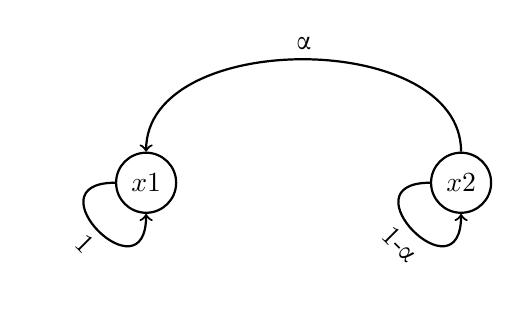
\begin{tikzpicture}[node distance={40mm}, thick, main/.style = {draw, circle}] 
		\node[main] (1) {$x1$};
		\node[main] (2) [right of=1] {$x2$};	
		
		\draw[->] (1) to [out=180,in=270,looseness=5] node [midway,below,sloped] {1} (1);
		\draw[->] (2) to [out=90,in=90,looseness=1] node [midway,above,sloped] {a} (1);
		\draw[->] (2) to [out=180,in=270,looseness=5] node [midway,below,sloped] {1-a} (2);
		\end{tikzpicture} \\ \\
	Όσον αφορά τη συνεκτικότητα του γραφηματος, το γράφημα είναι \textbf{ασθενώς συνεκτικό} καθώς δεν υπάρχει διαδρομή από τη κορυφή {\en x1} στη κορυφή {\en x2}. Για να ήταν ισχυρά συνεκτικό θα έπρεπε να υπήρχε διαδρομή από και προς όλες τις κορυφές του γραφήματος. \\ \\
	
	\pagebreak
	
	\textbf{4}. Ο αλγόριθμος ως συνάρτηση των αρχικών τιμών των παικτών \textbf{συγκλίνει κάθε φορά στο {\en x1}}.\\
	
	Αυτό ισχύει διότι:\\
	
	 \unboldmath{$\begin{bmatrix} x1 \\ x2 \end{bmatrix}$ = $x1 * \begin{bmatrix} 1 \\ 1 \end{bmatrix}  + (x2 - x1) * \begin{bmatrix} 0 \\ 1 \end{bmatrix}$} , όπου {\en v1} = $\begin{bmatrix} 1 \\ 1 \end{bmatrix}$ και {\en v2} = $\begin{bmatrix} 0 \\ 1 \end{bmatrix}$ τα ιδιοδιανύσματα από τα προηγούμενα \\ \\ ερωτήματα.\\
	 
	 Παίρνοντας το $\lim_{n \to \infty} A^{n} * \begin{bmatrix} x1 \\ x2 \end{bmatrix}$ έχουμε : \\
	 
	 $ A^{n} * \begin{bmatrix} x1 \\ x2 \end{bmatrix}$ = $ A^{n}*x1*v1 + A^{n}*(x2 - x1)*v2 = \lambda 1^{n}*x1*v1 + \lambda 2^{n}*(x2-x1)*v2$   (1) \\ \\, όπου $\lambda 1 = 1$ και $\lambda 2 = 1-\alpha$ \\ 
	 
	 Έχουμε ότι : $|1-\alpha| < 1$ οπότε $\lim_{n \to \infty} (1-\alpha)^n = 0$ και  $\lim_{n \to \infty} \lambda1^n = 1$.\\
	 Συνεπώς από την (1) $\Longrightarrow$ $\lim_{n \to \infty} (x1 * v1) = \begin{bmatrix} x1 \\ x1 \end{bmatrix}$
	
 
	\section*{\gr \textbf{Β.Θεωρητική Άσκηση 2}}
	
	\begin{enumerate}
	
	\item \par Για να απαντηθεί σωστά το ερώτημα θα πρέπει αρχικά να γίνει κατανοητό τι συμβαίνει στο {\en blockchain} τη στιγμή που υποβληθεί μία διπλοξοδευμένη συναλλαγή στο δίκτυο.  
	\par Εκείνη τη στιγμή δημιουργείται στο δίκτυο ένα {\en fork}.Ένα {\en fork} δημιουργείται όταν δυο {\en miners} τυχαίνει να εγκρίνουν ταυτόχρονα ένα {\en block} συναλλαγών και έτσι η αλυσίδα ενημερώνεται προς 2 κατευθύνσεις δημιουργώντας πολλαπλά προβλήματα στο δίκτυο. Έτσι για να αφαιρεθεί το {\en fork} οι {\en miners} δουλέυουν για να επεκτείνουν αυτό που είναι μεγαλύτερο στο δικό τους αντίγραφο του {\en blockchain}, ως ότου εγκριθεί η συναλλαγή.  
	
	Στη περίπτωση της άσκησης παρατηρούμε πως τη μεγαλύτερη υπολογιστική δύναμη την έχουν οι {\en miners} που δουλεύουν την υλοποίηση Α(80\% έναντι 20\% της Β). Συνεπώς συνεχίζουν να δουλεύουν στην υλοποίηση Α επεκτείνοντας την αλυσίδα του, κάνοντάς τη μεγαλύτερη από τη αλυσίδα του {\en blockchain } της υλοποίησης Β. Αυτό έχει ως αποτέλεσμα να μετακινηθούν οι {\en miners} της Β στην Α και κατά συνέπεια να οριστικοποιηθεί το {\en double-spending}.
	
	\item Σε αντίθεση με το υποερώτημα 1, τώρα 20\% της υπολογιστικής ισχύος τρέχει την υλοποιήση Α και 80\% την Β. Συνεπώς η υλοποίηση Β θα έχει μεγαλύτερη αλυσίδα και έτσι οι {\en miners} καταλαβαίνουν πως η συγκεκριμένη συναλλαγή αφορά {\en double-spending} και προχωρούν στην αναγνώριση της ως άκυρη.
	\end{enumerate}
	
	\section*{\gr \textbf{Γ.Θεωρητική Άσκηση 3}}
	
	Ο Μπομπ \textbf{δεν πρέπει} να δεχτεί το πρωτόκκολο της υπόθεσης.\\ \\ Καταλήγουμε στο συγκεκριμένο συμπέρασμα καθώς παρατηρούμε πως η Αλίκη μπορεί να στείλει το {\en s} στο {\en C{\scriptsize M}} μετά από χρόνο 2Δ και να πάρει το επιτυχώς το πράσινο νόμισμα, και ταυτόχρονα ο Μπομπ να μην μπορεί να στείλει το {\en s} στο {\en C{\scriptsize A}} καθώς ο χρόνος 2Δ θα έχει ήδη τελείωσει. \\
	
	
	\section*{\gr \textbf{Δ.Προγραμματιστική Άσκηση 1}}
	
	Τα κουμπιά που χρησιμοποιούμε είναι τα : {\en strategy}(Οι 4 περιπτώσεις) , {\en n} (Αριθμός Κόμβων).\\
	
		\begin{center}
		\textbf{Περίπτωση 1} : Όλοι οι κόμβοι συγκλίνουν στο μέσο όρο τους.  
		\begin{figure}[h]
			\centering 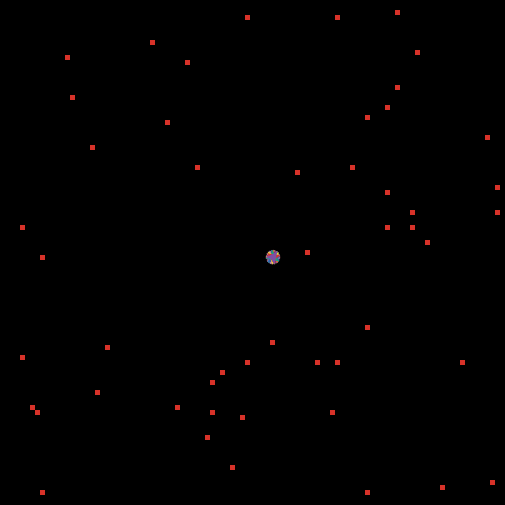
\includegraphics[scale=0.40]{pics/Friedkin-Johnsen_model view.png}  
		\end{figure}
		\pagebreak
		
		\textbf{Περίπτωση 2} : Όλοι οι κόμβοι παραμένουν στις αρχικές τους θέσεις.
		 \begin{figure}[h] 
		 	\centering 
\includegraphics[scale=0.40]{pics/Friedkin-Johnsen_model view2.png} 
	 	 \end{figure}
		
		\textbf{Περίπτωση 3} : Οι κόμβοι που δεν επιμένουν στην αποψή τους αρχικά συγκλίνουν στο μέσο όρο όλων των κόμβων και σταδιακά μετακινούνται προς την άποψη του κόμβου που επιμένει. 
		\begin{figure}[h]
		 \centering 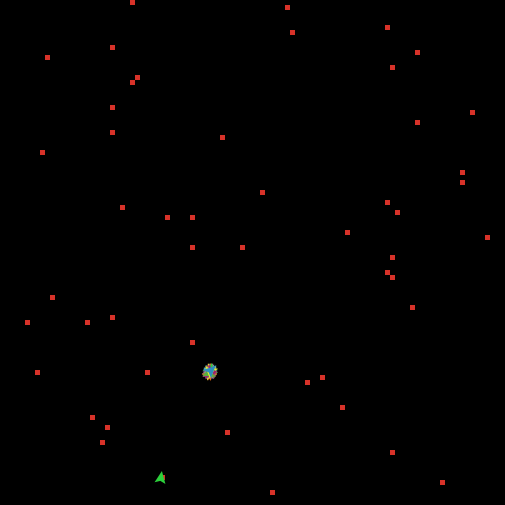
\includegraphics[scale=0.40]{pics/Friedkin-Johnsen_model view3.png} 
		\end{figure}
	
		\pagebreak
	
		\textbf{Περίπτωση 4} : Κάθε κόμβος συγκλίνει σε διαφορετικό σημείο.Κόμβοι με μεγάλο θ συγκλίνουν κοντά στην αρχική τους θέση ενώ κόμβοι με μικρό θ συγκλίνουν προς το μέσο όρο των κόμβων.
		 \begin{figure}[h]
		\centering 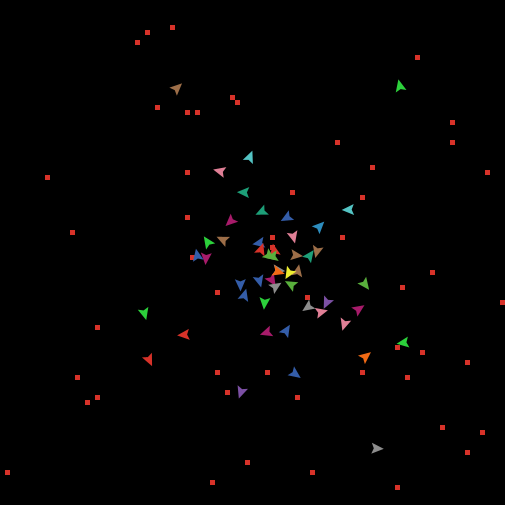
\includegraphics[scale=0.40]{pics/Friedkin-Johnsen_model view4.png} 
		\end{figure}
		\end{center}
		
		
		
	\section*{\gr \textbf{E.Προγραμματιστική Άσκηση 2}}
	
	Ο πειραματικός υπολογισμός της κρίσιμης πιθανότητας πραγματοποιήθηκε αξιοποιώντας το {\en plot Critical chance} που δημιουργήθηκε. Τα αποτελέσματα που εξάχθηκαν για τη κρίσιμη πιθανότητα σε κάθε ερώτημα είναι τα εξής: \\
	
	\textbf{Ερώτημα 1:}
	\begin{itemize}
		\item Απλή γειτονιά {\en Moore }: κρίσιμη πιθανότητα στο 39\% {\en tree density}.
	\end{itemize}
	 
	 \textbf{Ερώτημα 2:}
	 \begin{itemize}
	 \item Απλή γειτονιά {\en Moore }: κρίσιμη πιθανότητα στο 43\% {\en tree density}. 
	 \item Γειτονιά {\en Moore }με τρία τουλάχιστον δένδρα να καίγονται: Δεν παρατηρούμε κάποια ιδιαίτερη συμπεριφορά. Κρίσιμη πιθανότητα στο 94\% {\en tree density}.
	 \item Γειτονιά {\en Moore }με τρία τουλάχιστον δένδρα να καίγονται: Δεν καίγεται κανένα δένδρο μέχρι το {\en tree density} φτάσει στο 95\% . 
	 \end{itemize}
 
 	\textbf{Ερώτημα 3:}
 	\begin{itemize}
 		\item Για {\en wind = 1}: κρίσιμη πιθανότητα στο 38\% {\en tree density}. 
 		\item Για {\en wind = 2}: κρίσιμη πιθανότητα στο 27\% {\en tree density}. 
 	\end{itemize}
 
 	\textbf{Ερώτημα 4:}
 	\begin{itemize}
 		\item Για {\en q = 60\%}: κρίσιμη πιθανότητα στο 71\% {\en tree density}. 
 		\item Για {\en q = 90\%}: κρίσιμη πιθανότητα στο 62\% {\en tree density}. 
 	\end{itemize}
 
 	\textbf{Ερώτημα 5:}
 	\begin{itemize}
 		\item Για {\en q = 60\%} και {\en phard = 50\%}: κρίσιμη πιθανότητα στο 68\% {\en tree density}. 
 		\item Για {\en q = 60\%} και {\en phard = 100\%}: κρίσιμη πιθανότητα στο 65\% {\en tree density}. 
 		\item Για {\en q = 90\%} και {\en phard = 50\%}: κρίσιμη πιθανότητα στο 62\% {\en tree density}. 
 		\item Για {\en q = 90\%} και {\en phard = 100\%}: κρίσιμη πιθανότητα στο 61\% {\en tree density}.
 	\end{itemize}
 
 	\textbf{Ερώτημα 6:}
 	\begin{itemize}
 		\item Για {\en wind = 0}: κρίσιμη πιθανότητα στο 61\% {\en tree density}. 
 		\item Για {\en wind = 1}: κρίσιμη πιθανότητα στο 42\% {\en tree density}. 
 		\item Για {\en wind = 2}: κρίσιμη πιθανότητα στο 42\% {\en tree density}.Εδώ το αποτέλεσμα είναι ίδιο με τη παραπάνω περίπτωση διότι ο αγροτικός δρόμος είναι σαν μην υπάρχει λόγω ανέμου.
 	\end{itemize}
 
	\textbf{Ερώτημα 1:}
	\begin{itemize}
	\item {\en Moore = ON} , {\en wind = 2} , {\en q = 0.5} , {\en phard = 0.5} , {\en farmer road = ON}: κρίσιμη πιθανότητα στο 31\% {\en tree density}. \\ 
 	\end{itemize}
\end{document}